\documentclass[10pt]{article}
\usepackage[utf8]{inputenc}
\usepackage{geometry}
\usepackage[T1]{fontenc}
\usepackage{amsfonts}
\usepackage{graphicx}
\usepackage{float}
\usepackage{hyperref}
\usepackage[sorting=none]{biblatex}
\usepackage{fancyhdr}
\usepackage{multicol}
\usepackage{utopia}
\addbibresource{ref.bib}
\fontfamily{put}\selectfont
\setlength{\columnsep}{40pt}
\setlength{\voffset}{0.5cm}
\setlength{\headsep}{40pt}
\geometry{legalpaper, portrait, margin=2.3cm}

\bibliography{ref.bib}


% Title page
\title{Project:\\ \textbf{Hot and Cold Rubidium}\\\Large{ Dr. Pablo Solano Palma \\ 2024}}
\author{ Nicolas Vera, Amaru Moya, Enrique Orellana, Omar, Florencia, etc. \ Universidad de Concepción\\ Faculty of Physical and Mathematical Sciences, Physics Department}
% \date{\today}

% Header and footer
\pagestyle{fancy}
\fancyhead[C]{
\includegraphics[width=0.05\textwidth]{img/escudo.png}}
\fancyhead[L]{\textbf{Thesis Project}\\ Universidad de Concepción}
\fancyhead[R]{\textbf{Amaru Moya R.}\\ amarumoya@udec.cl}
\fancyfoot{}
\begin{document}

\maketitle
\thispagestyle{fancy}




\clearpage
% \tableofcontents
% \thispagestyle{fancy}

% \clearpage
% Begin page numbers
\fancyfoot[C]{\thepage}
\pagenumbering{arabic}
% \begin{multicols}{2}

% pq es interesante, como contribuye con el entendimiento de la naturaleza del ser humano
% estado del arte/ grupos que estudien tematicas similares?
% que evidencia hay que este proyecto pueda resolver el problema planteado?
% compatibilidad en los recursos, tiempos y problemas


% estado del arte y fundamentos,% revision de conceptos tecnicos

% preguntas hipotesis y objetivos, potencial impacto

% marco metodologico, objetivos

\section*{Summary}
\addcontentsline{toc}{section}{Introduction} % For the contents page

% Describa los principales temas que se abordarán en el proyecto: objetivos, metodología y resultados esperados. La extensión máxima de esta sección es de 1 página (utilizar formato tamaño carta, fuente Verdana tamaño 10 o similar).


\noindent The main objective of this project is to study and manipulate the index of refraction of a Rubidium vapour through the interaction with laser light of two different wavelengths. Using a theoretical, numerical and experimental approach, we aim to understand and characterize the Rubidium vapour and the effects of light interacting with this system. The project will be divided into three main stages: theoretical study, numerical simulations, and experimental validation. The theoretical study will focus on the fundamentals of atomic quantum optics, with emphasis on the interaction between light and matter. The numerical simulations will be used to model the interaction between light and Rubidium vapour, and to predict the behaviour of the system under different conditions. Finally, the experimental validation will involve the construction of an experimental setup to measure the index of refraction of the Rubidium vapour and compare the results with the theoretical and numerical predictions. The expected results of this project include a better understanding of the interaction between light and matter, and the development of new techniques for manipulating the index of refraction of Rubidium vapour. This research has the potential to have a significant impact on the field of quantum optics and quantum information processing, and to open up new possibilities for the development of quantum technologies.


\newpage
\section*{Rubidium}
\subsection*{Atomic Structure}
% Rb Structure, Dlines, 

\section*{Laser 1}

\begin{figure}
    \centering
    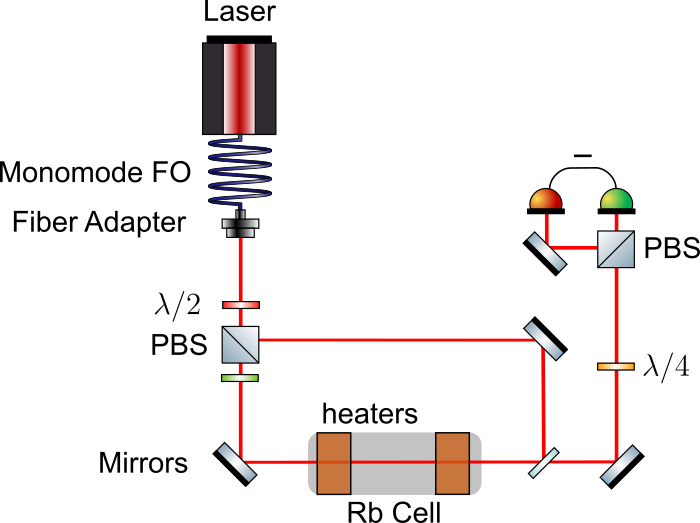
\includegraphics[width=0.5\textwidth]{img/rect5909.png}
    \caption{Set up for Laser 1}
    \label{fig:laser1}
\end{figure}

\begin{enumerate}
    \item Osciloscope
    \item Signal Generator
    \item TEC: Temperature Controller
    \item Control of Control
    \item Laser Control
    \item Current Control %(Coil de la válvula)
    \item Rubidium Heater for Glass Cell
\end{enumerate}

\section*{Laser 2}

\section*{Laser 3}


\section*{Bragg Reflections in Rubidium Vapours}

\subsection*{Objectives}


\subsection*{Experimental Set Up}
Rubidium Borosilicate Reference Cell, Ø25.4 mm x 71.8 mm %GC25075-RB	
SM1FCA - FC/APC Fiber Adapter Plate with External SM1 (1.035"-40) Threads, Wide Key (2.2 mm) 



\section*{Bragg Reflections in Cold Rubidium}
\subsection*{Objectives}



\subsection*{Experimental Set Up}

\newpage
\section*{References}

% Incluya en esta sección, el listado de referencias bibliográficas completas citadas en la sección Formulación de la Propuesta. Extensión: 2 páginas (utilizar formato tamaño carta, fuente Verdana tamaño 10 o similar).

% por lo menos 20 que tengo que manejar bien


\end{document}
